\section{Evaluation von Datenanalyseverfahren}

\subsection{Training und Testing}
Es ist üblich, den verfügbaren Datenbestand in einem 2:1 Verhältnis aufzuteilen,
wobei der größere Teil als Trainingsdatenbestand für den zu bewertenden Classifier
verwendet wird. Um nun den resultierenden Classifier testen zu können, wird der
Rest der Daten als so genannter Testdatenbestand eingesetzt.
\textit{Nach} dem Testen können die Testdaten zusammen mit den Trainingsdaten zur 
Verfeinerung des Classifiers verwendet werden.

Es ist auch eine Unterteilung in \textit{Trainings-, Validierungs-} und 
\textit{Testdaten} denkbar, bei der die Validierungsdaten vor allem zur Parametereinstellung
verwendet werden. 

Möchte man auf eine Unterteilung der Daten verzichten, und benutzt alle Daten für
die Erstellung des Classifiers, so ist dies im Allgemeinen kein gutes Vorgehen,
da man nicht mehr viel über die Güte aussagen kann. Ein Ansatz wäre es, die
Fehlerrate des Classifiers angewandt auf den Trainingsdatenbestand zu berechnen,
was jedoch keine besonders hohen Wert hat, da diese Daten ja schon zum Erstellen des
Classifiers verwendet wurden.

Ein wichtiger Aspekt ist die Verteilung der Klassenzugehörigkeiten innerhalb der
verschiedenen Partitionen. Diese sollte in etwa gleich sein über alle Partitionen
hinweg. Dieser Vorgang der Homogenisierung nennt sich \textbf{Stratification}.
Der Sinn dahinter ist, Fehler möglichst zuverlässig abschätzen zu können. 
Es könnte nämlich bei einer randomisierten Partitionierung der Fall 
auftreten, dass die Trainingsdaten krass von den Testdaten abweichen (Ausreißer) 
und dadurch der Classifier falsche Vorhersagen liefert.

Oft ist unsere Ausgangssituation die, dass uns nur wenig Daten zur Verfügung
stehen. Um trotzdem eine gute Evaluation unseres Classifiers zu erhalten, gibt es
das Verfahren der \textbf{Crossvalidation}. Die Grundidee beruht auf der 
\textit{repeated holdout method}: Es werden die Daten zufällig aufgeteilt in
Trainings- und Testdaten und daraus die Fehlerrate berechnet. Dies wird mehrmals
wiederholt und am Ende wird der Durchschnitt aus den Fehlerraten berechnet.
Bei der Crossvalidation wird eine fixe Anzahl an Partitionen generiert, sogenannte
\textit{Folds}. Einer dieser Folds wird für das Testen verwendet, der Rest als
Trainingsdaten. Bei jeder Iteration wird nun die Testpartition gewechselt.
Auch bei der Crossvalidierung kann eine Stratification sinnvoll sein, um die
Varianz und die Verzerrung des Ermittelten Fehlers zu verringern. Der Standard
ist eine \textit{10-fold Crossvalidation}.

\subsection{Wahrscheinlichkeiten als Vorhersageergebnis}
Da es im Allgemeinen besser ist, eine Wahrscheinlichkeit als Classifier-Ergebnis
zu erhalten (z.B. Kunde ist zu 87\% kreditwürdig), sollte dies auch irgendwie in
der Evaluation berücksichtigt werden. Dies geschieht meist durch Berechnung der
Verluste, die bei einer falschen Vorhersage auftreten. Die Grundform einer
\textbf{Loss Function} gibt an, wie viel man bei unkorrekter Vorhersage verliert
(die Art des Fehlers und daraus resultierende unterschiedliche Kosten werden hier
noch nicht berücksichtigt). Beispiel einer 0-1 Loss Function:
\[
	Loss_{0-1} = 
		\begin{cases}
			0 &\quad \text{wenn Vorhersage richtig,}\\
			1 &\quad \text{ansonsten.}\\
		\end{cases}
\]

Dies entspricht unserer bisherigen Betrachtungsweise, es gibt nur "'schwarz-weiß"'.
Im Folgenden werden wir uns mit den Grautönen beschäftigen.

Eine Erweiterung der \(Loss_{0-1}\)-Function
ist die \textbf{Quadratic Loss Function}. Es sei \(k\) die Anzahl
an Klassen. Damit liefert der Classifier für ein Datenobjekt
einen Ergebnisvektor \((p_1 , \dots , p_k)\),
der sich zu 1 aufsummiert
(z.B. Ergebnis des Classifiers: Person ist zu 87\% guter Kunde und zu 13\% schlechter
Kunde). Die tatsächliche Klassenzugehörigkeit eines Objektes lässt sich als
Vektor \((a_1, \dots , a_k)\) darstellen, wobei, an der \(i\)-ten Stelle eine 1 steht,
wenn das Objekt zu Klasse \(i\) gehört.
Damit ergibt sich die Quadratic Loss Function als
\[
	QLoss = \sum_{j=1}^k (p_j - a_j)^2.
\]
Hätte man einen Classifier, der komplett daneben liegt, also z.B. Vorhersage \((0,1)\)
obwohl wahre Klassenzugehörigkeit \((1,0)\) ist, dann ergibt sich der maximale Loss als
\textbf{2}. Um den Quadratic Loss zu minimieren, ist es am besten, wenn die 
Wahrscheinlichkeiten insgesamt möglichst gleich sind.

Ein weiteres Maß ist der \textbf{Informational Loss}, der sich mit 
\[
	LogLoss = -\log_2 (p_i)
\]
berechnen lässt, wobei hier \(i\) die korrekte Klasse ist.
Da der Logarithmus nicht für \(0\) definiert ist, sollte damit
unser Schätzer auch nie eine Klasse mit der Wahrscheinlichkeit von \(0\%\) vorhersagen,
da sonst unser Loss unendlich groß würde.\footnote{Auch als \textit{zero-frequency-problem}
bekannt}

Im Vergleich ist der Quadratic Loss aussagekräftiger, da er alle Ergebnisse verwertet,
und nicht nur eine Spalte betrachtet, wie der Informational Loss. Letzterer
kann jedoch nützlich sein, wenn man nur an dem Ergebnis bzgl. einer bestimmten
Klassenzugehörigkeit interessiert ist.

\subsection{Fehlerarten und entsprechende Maße}
\subsubsection{Bias vs. Varianz}
\textbf{Bias} ist die Verzerrung, also wie weit der berechnete Wert vom tatsächlichen
abweicht (z.B. Mittelwert im Trainingsdatenbestand ist doppelt so groß, wie der
wahre Wert). Die \textbf{Varianz} ist die Streuung um den ermittelten Wert.

Unterliegt unser Classifier einer Verzerrung, so ist dieser Fehler beim Lernen
\textit{konsistent}, d.h. auch bei einem unendlichen großem Trainingsdatenbestand
verschwindet er nicht. Die Varianz ist der Fehler, der durch die begrenzte Anzahl
der Trainingsdaten entsteht; wird die Varianz sehr groß, so bedeutet dies ein
\textit{Overfitting}: Es wird nicht mehr die vorgesehen Ausgabe modelliert, sondern
das Rauschen in den Trainingsdaten.

Mithilfe der \textit{Bias-Variance-Decomposition} kann der erwartete Fehler 
analysiert werden, der aus 3 Teilen besteht: Dem Bias, der Varianz und dem
irreduziblen Fehler, resultierend aus dem Rauschen innerhalb der Daten selbst.

\subsubsection{Fehlerarten und Erfolgsquote}
Im Wesentlichen lässt sich zwischen 2 Fehlerarten unterscheiden, den 
\textbf{False Positives} und den \textbf{False Negatives}, wobei letztere auch als
\textit{misses} bezeichnet werden. Die Gesamt-Erfolgsquote ergibt sich aus
\[
	\frac{TP+TN}{TP+TN+FP+FN} = \frac{\text{Anzahl der richtigen Vorhersagen}}
	{\text{Anzahl aller Vorhersagen}}
\]
Die Ergebnisse eines Klassifikators lassen sich durch eine so genannte
\textit{Konfusionsmatrix} darstellen. So repräsentieren die Zeilen die tatsächlichen
Klassen, und die Spalten stellen die vorhergesagten Klassen dar. In der ersten Diagonalen
steht die Anzahl der jeweils korrekt vorhergesagten Klasse.

Um 2 Klassifikatoren miteinander zu vergleichen, kann man den \textbf{Kappa-Koeffizienten}
zu Rate ziehen. 
\begin{quote}
	\glqq The Kappa statistic (or value) is a metric that compares an Observed Accuracy 
	with an Expected Accuracy (random chance). The kappa statistic is used not only
	to evaluate a single classifier, but also to evaluate classifiers amongst 
	themselves. In addition, it takes into account random chance (agreement with a 
	random classifier), which generally means it is less misleading than simply 
	using accuracy as a metric (an Observed Accuracy of 80\% is a lot less 
	impressive with an Expected Accuracy of 75\% versus an
	Expected Accuracy of 50\%).\grqq
\end{quote}
Amazing.\footnote{\url{http://stats.stackexchange.com/questions/82162/kappa-statistic-in-plain-english}}
Formaler ausgedrückt ist der Kappa-Koeffizient also
\[
	\kappa =  \frac{\text{Number of observed successes} - 
	\text{Number of expected successes}}{\text{Total number of possible successes} -
	\text{Number of expected sucsesses}}
\]
Dieser Koeffizient wird maximal, wenn unser Ausgangs-Classifier immer richtig liegt,
also \(\kappa = 1\). Wenn unser Classifier immer daneben liegt, dann kann \(\kappa\)
unter Umständen sehr klein werden, ist also nach unten nicht beschränkt. Ein weiteres
Phänomen, das auftreten kann, ist, dass unser Classifier Objekte nicht öfter richtig 
vorhersagt, als naives Raten; unser Classifier ist also gerade so
gut, wie es der Zufall auch ist, also nicht wirklich erstrebenswert. In diesem Fall
ist \(\kappa = 0\). Im Allgemeinen ist die Qualifizierung des Koeffizienten eher
willkürlich, es gibt dafür verschiedene Ansätze. Außerdem sollte stets eine 
Konfusionsmatrix bei der Interpretation betrachtet werden. Für ein Beispiel, siehe
Fußnote.

\subsection{Lift Charts}
Als Beispiel betrachten wir das Verschicken von Werbeflyern an viele Haushalte. Im Allgemeinen
gibt es nur wenige Antworten, in etwa \(0.1\%\). Es kann aber der Fall sein, dass
es einen Landkreis gibt, aus dem besonders viele Antworten stammen. Würde man nun
nur noch dieses Landkreis anschreiben, so könnte sich die Antwortrate auf etwa
\(0.5\%\) erhöhen. Es wäre wohl also sinnvoll, sich bei seinem Marketing vor allem
auf dieses Gebiet zu konzentrieren. Diese Erhöhungsfaktor nennt sich
\textbf{Lift} und hat in diesem Beispiel den Wert 5. 
\begin{figure}[ht]
	\subfigure{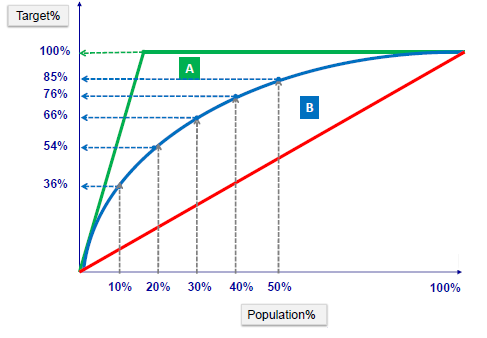
\includegraphics[width=0.49\textwidth]{Figures/gain_chart}}
	\subfigure{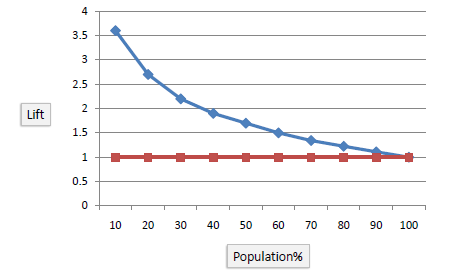
\includegraphics[width=0.49\textwidth]{Figures/lift_chart}}
	\caption{Quelle: \href{http://www.saedsayad.com/model_evaluation_c.htm}{www.saesdsayad.com}}
	\label{fig:lift}
\end{figure}

\noindent In Abb.~\ref{fig:lift}  kann man die Wirkung des Lifts gut erkennen.
Die grüne Kurve A zeigt, dass es ab ca. \(15\%\) der gesamten Population keinen Sinn
mehr macht, mehr Leute anzuschreiben, da keine weiteren Responses mehr hinzukommen.
Die Blaue Kurve B zeigt, dass, obwohl es noch einen Zuwachs an Responses gibt, 
dies nur noch in relativ geringem Maße stattfindet. Rechts daneben ist in einem
Lift Chart dargestellt, welchen Wert der Lift bei welcher Population annimmt.

\subsection{ROC Kurven}
Eine weitere Bewertungsgrundlage sind die \textbf{ROC-Kurven} (receiver operating
characteristics). Diese basieren auf ein paar Grundlegenden Kennzahlen beruhen,
nämlich
\begin{align*}
	&\text{False Positive Rate } &100\% \cdot \frac{FP}{FP+TN}\\
	&\text{True Positive Rate (Recall) } &100\% \cdot \frac{TP}{TP+FN}\\
\end{align*}
Wählt man die False Positive Rate als x-Achse und trägt auf die y-Achse den Recall
ein, so kann man die beiden im Verhältnis zu einander in einem Graphen darstellen
wie in Abb.~\ref{fig:roc}.

\begin{figure}[ht]
	\centering
	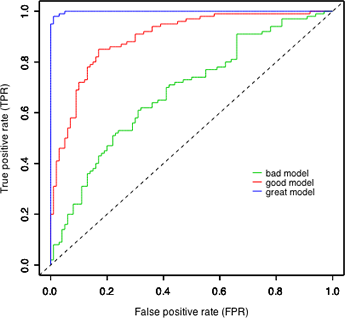
\includegraphics[width=0.625\textwidth]{Figures/roc_curve}
	\caption[ROC Curve]{Beispiel einer ROC Kurve mit FP-Rate und Recall als Achsen.\footnotemark}
	\label{fig:roc}
\end{figure}
\footnotetext{https://www.unc.edu/courses/2010fall/ecol/563/001/docs/lectures/lecture22.htm}

Anstelle des Recalls kann man auch die \textbf{Precision} als y-Achse verwenden,
die sich aus 
\begin{align*}
&\text{Precision } &100\% \cdot \frac{TP}{TP+FP}\\
\end{align*}
ergibt.

Im Graphen ist es, wie bei einem Gain Chart, besser, wenn der Graph möglichst weit
oben links verläuft, da dann bei nur geringer False Positive Rate bereits eine
sehr hohe Recall-Rate erreicht wird. Befindet man sich unten rechts, so ist das
Ergebnis dementsprechende schlechter.

Um nun die ROC Kurve quantifizieren zu können, wir meist die Fläche unter der
Kurve (\textbf{AUC}) betrachtet. Analog lassen sich auch andere Maße verwenden,
wie etwa der \textbf{11-point average recall}\footnote{Oder auch Precision.}.
Hierbei wird an den Stellen 0\%, 10\%, ... 100\% der Wert gemessen und aus allen
der Durchschnitt berechnet.

Weitere Kennzahlen, die beide Fehlerarten berücksichtigen, sind das 
\textbf{f-Measure} (F1-score) und die \textbf{Erfolgsquote}. Die 
Erfolgsquote ist einfach die Anzahl aller richtigen Vorhersagen geteilt durch die
Anzahl aller Vorhersagen, also
\[
	\frac{TP+TN}{TP+FP+TN+FN}.
\]
Das f-Measure ist das harmonische Mittel der Precision und des Recalls:
\[
	2 \cdot \frac{recall \cdot precision}{recall + precision}
\]
Die Multiplikation mit 2 sorgt dafür, dass das f-Measure den Wert 1 annimmt,
wenn sowohl Precision als auch Recall den Wert 1 haben. Die Allgemeine Form
lautet:

\[
	F_\beta = (1 + \beta ^2) \cdot \frac{precision \cdot recall}{(\beta^2 \cdot precision) + recall}
\]

\begin{quote}
	\glqq The F-measure was derived, so that \(F_\beta\) 
	measures the effectiveness of retrieval
	with respect to a user who attaches \(\beta\) times as much impartance to recall as 
	precision.\grqq
	\footnote{\href{https://en.wikipedia.org/wiki/F1_score}{wikipedia.com}}
\end{quote}

\begin{figure}[ht]
	\centering
	\begin{tikzpicture}
		\draw [->] (0,0) -- (10,0);
		\draw [->] (0,0) -- (0,10);
		\draw [dotted] (0,10) -- (10,10);
		\node [below] at (5,-0.5) {\(p[+]\)};
		\node [left] at (-0.5,5) {\(\epsilon\)};
		\node [below left] at (0,0) {\(0\)};
		\node [left] at (0,10) {1};
		\node [below] at (10,0) {1};
		\node [right] at (6,9) {Always wrong};
		\node [right] at (6,1) {Always right};
		\node [below] at (2,7) {Always pick +};
		\node [right] at (8,7) {Always pick -};
		\draw [arrows = {-Stealth[]}] (6,1) -- (5,0); 
		\draw [arrows = {-Stealth[]}] (6,9) -- (5,10);
		\draw [blue, arrows = {-Stealth[]}] (8,7) -- (7,7);
		\draw [red, arrows = {-Stealth[]}] (2,7) -- (2,8);
		\draw [dashed, blue] (0,0) -- (10,10);
		\draw [dashed, red] (0,10) -- (10,0);
		\draw [thick] (0,2) -- (10,5);
		\node [right] at (10,5) {A};
		\draw [<->] (-0.2, 0.3) -- (-0.2,1.7);
		\node [] at (-0.5,1) {\(f_p\)};
		\draw [<->] (10.2,0.3) -- (10.2,4.7);
		\node [] at (10.5,2.5) {\(f_n\)};
	\end{tikzpicture}
	\caption{Eine alternative Darstellung von erwartetem Fehler 
	\(\epsilon\) im Verhältnis zur
	Wahrscheinlichkeit \(p[+]\), dass ein zufälliges Objekt zur Klasse \([+]\) 
	gehört.}
	\label{fig:alt}
\end{figure}


In Abb.~\ref{fig:alt} kann man die erwartete Fehlerquote eines Classifiers im
Verhältnis zu der Wahrscheinlichkeit, dass ein Objekt zu einer bestimmten Klasse
gehört, betrachten. Die Gerade eines Classifiers, der immer richtig liegt, entspricht
der x-Achse, da ja der erwartete Fehler gleich 0 ist. Rät der Classifier jedoch immer
falsch, so ist der Graph \(\epsilon = 1\). Die beiden Diagonalen repräsentieren 
jeweils einen Classifier, der für alle Objekte angibt, dass diese Teil (oder nicht Teil)
der Klasse \([+]\) sind. Gerade \textit{A} stellt einen moderateren Classifier dar. 
Die Formel für ihn lautet \(A = f_p \cdot (1-p) + f_n \cdot p\). \(f_p\) ist genau die 
False Positive Rate, da für \(p[+]=0\) keine Objekte zu der Klasse \([+]\) gehören
können. Entsprechend ist \(f_n\) die False Negative Rate. In diese Grafik können
auch ganz leicht die Kosten für die jeweiligen Fehlerarten eingeführt werden,
indem einfach die Summanden von \textit{A} mit den Kosten der entsprechenden Fehler
multipliziert werden, was offensichtlich wieder eine Gerade ergibt.

Im Großen und Ganzen soll Abb.~\ref{fig:alt} nur eine alternative 
Visualisierungsmöglichkeit präsentieren.

\begin{figure}[ht]
	\centering
	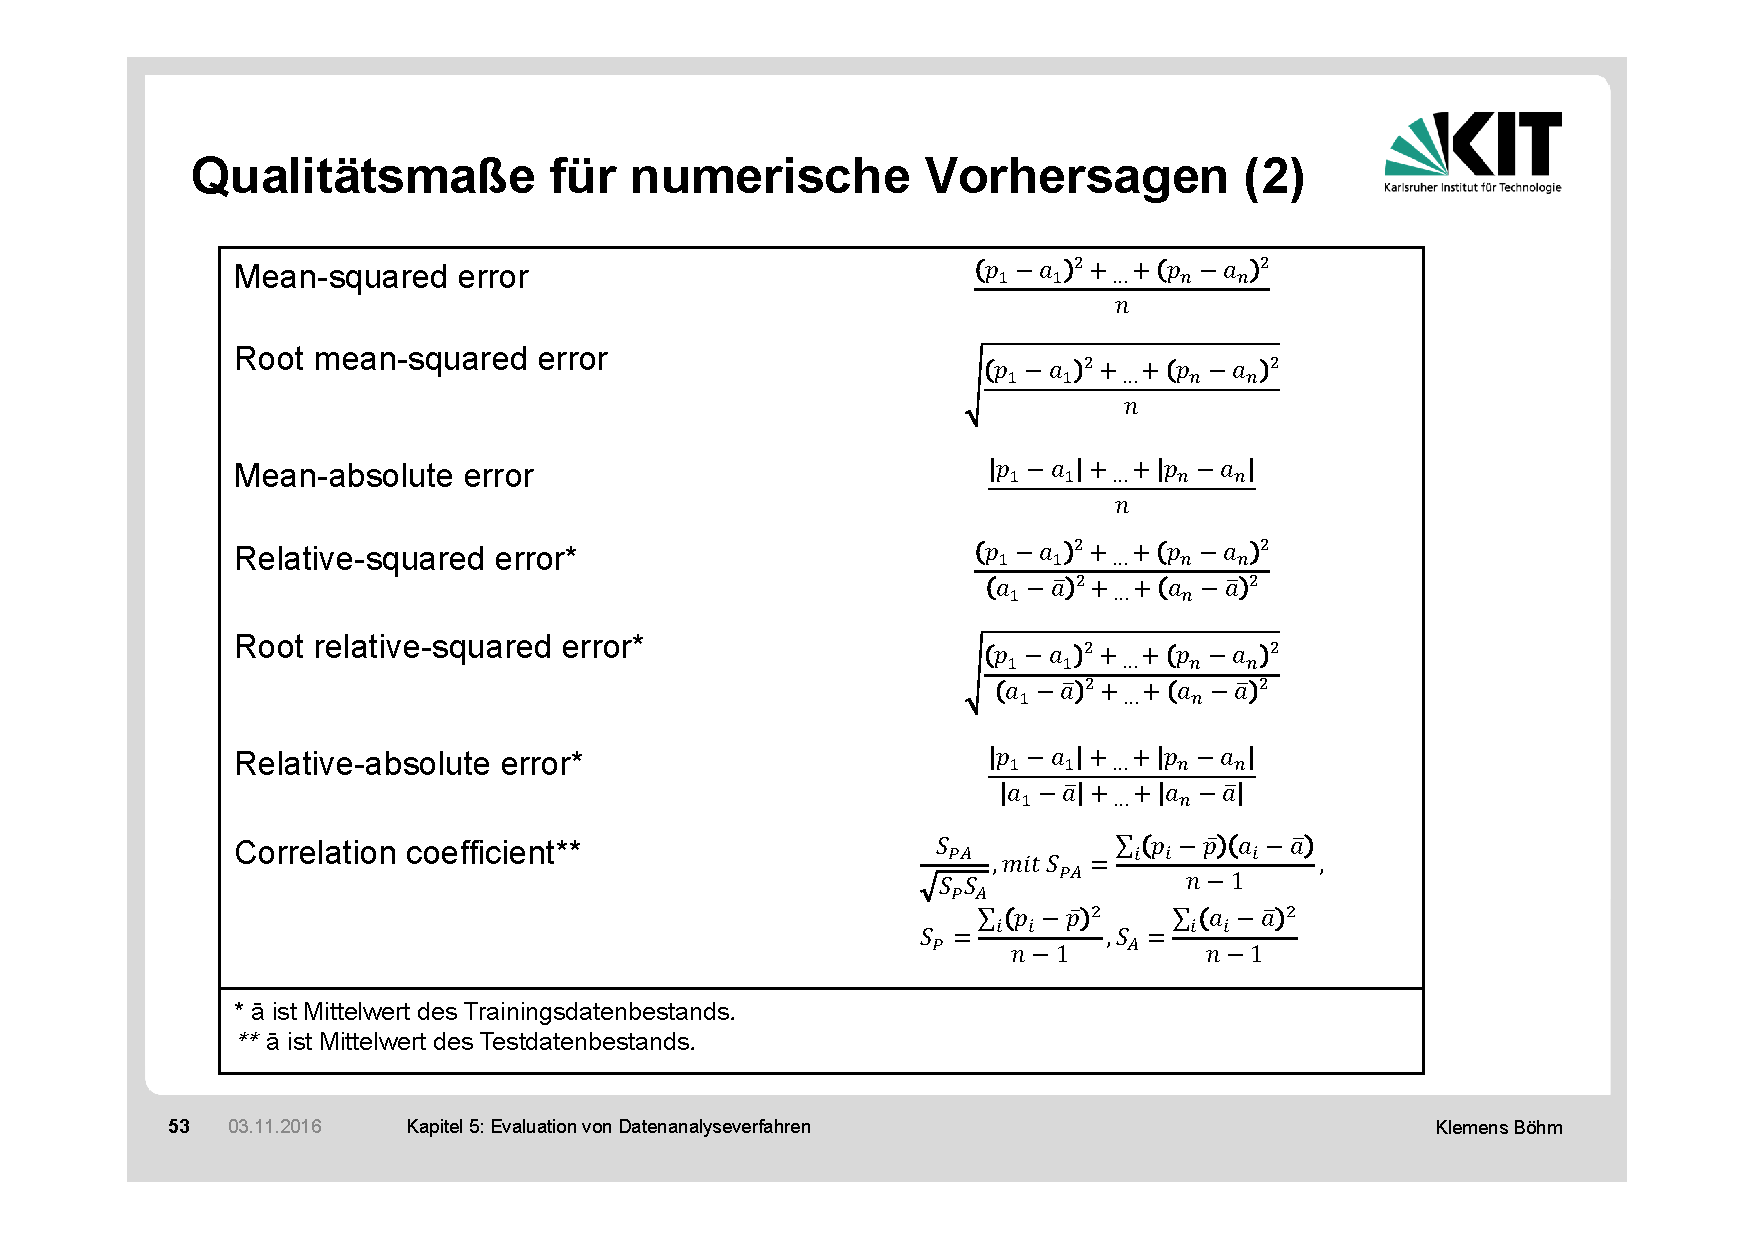
\includegraphics[width=\textwidth]{Figures/numeric_measures}
	\caption[Numeric Measures]{Verschiedene numerische Qualitätsmaße. Hierbei beschreibt
	\(p_i\) die Vorhersage für das \(i\)-te Obejkt im Trainingsdatenbestand
	und \(a_i\) ist der tatsächliche Wert.\footnotemark}
	\label{fig:numeric}
\end{figure}
\footnotetext{Foliensatz 5, S.53}

Wenn wir uns in den Raum der numerischen Vorhersage begeben, und nicht nur die 
einfache Klassenzugehörigkeit von Objekten voraussagen wollen, so kann man 
dies mit 3 Arten von Maßen quantifizieren, die in Abb.~\ref{fig:numeric} zu
sehen sind. Die ersten drei Kennzahlen liefern absolute Werte, sie sind also unter
Umständen schwer zu interpretieren. Besser wäre wohl ein \textit{relatives Maß}, welches mit
den nächsten drei Kennzahlen bewerkstelligt werden kann. Effektiv stehen bei diesen 
im Zähler die Werte unseres Classifiers und im Nenner ein simpleres Verfahren (hier
die Abweichung vom Mittelwert). Wird der Wert des Bruchs größer als 1, dann 
ist unser Classifier weniger effektiv, als wenn man einfach immer den Mittelwert
des Datenbestandes vorhergesagt hätte. Liegt jedoch ein perfekter fit vor, dann
ist der Wert des Bruches 0, der Wertebereich ist also \([0,\infty]\). Die letzte 
Kennzahl ist der \textit{Korrelationskoeffizient}, welcher die Gleichheit zweier
Verteilungen misst, in unserem Fall die Verteilung der Werte unseres Classifiers
und die der echten Werte. Der Wertebereich des Korrelationskoeffizienten ist
\([-1,1]\), minimal wird er, wenn eine \textit{negative} Korrelation vorliegt,
maximal, wenn eine Gleichheit der Verteilungen vorliegt und er wird 0, wenn überhaupt
keine Korrelation besteht.

\subsection{Minimum Description Language}
Zunächst ein paar Grundlagen.

\begin{itemize}
	\item \(X\) sei ein \textbf{Alphabet}
	\item \(C\) sei eine injektive Abbildung (\textbf{Code}) von \(X\) auf
		\(\{0,1\}^{+}\)
	\item \(L_c (x)\) sei die \textbf{Länge} (in Bits) der Beschreibung von x
\end{itemize}

Wenn \(\forall x: L_c(x)\) gleich ist, dann nennt man den Code \textbf{uniform}. Ziel soll
es sein, eine möglichst kurze Codierung zu finden. Kennt man die 
Wahrscheinlichkeitsverteilungen der Buchstaben, so kann man folgenden Zusammenhang
feststellen:
\[
	\forall x: L_c(x) = \lceil -\log P(x) \rceil
\]
Damit ergeben sich für häufige Buchstaben kurze Codierung und vice versae für seltene
Buchstaben. Der kürzest mögliche Code entsteht also, wenn die Längen der Codierungen
der Wahrscheinlichkeitsverteilung der Buchstaben gleichen.

Im Allgemeinen ist also die Berechnung der Code-Längen aus der Wahrscheinlichkeitsverteilung
(und auch umgekehrt) durchaus möglich.

\subsubsection{Minimum Message Length}
Ein mit dem MDL verwandtes Konzept ist MML, die Beschreibung von einem Datenbestand
mithilfe eines \textbf{Modells}. 

\begin{figure}
	\subfigure[Lineares Modell]{
		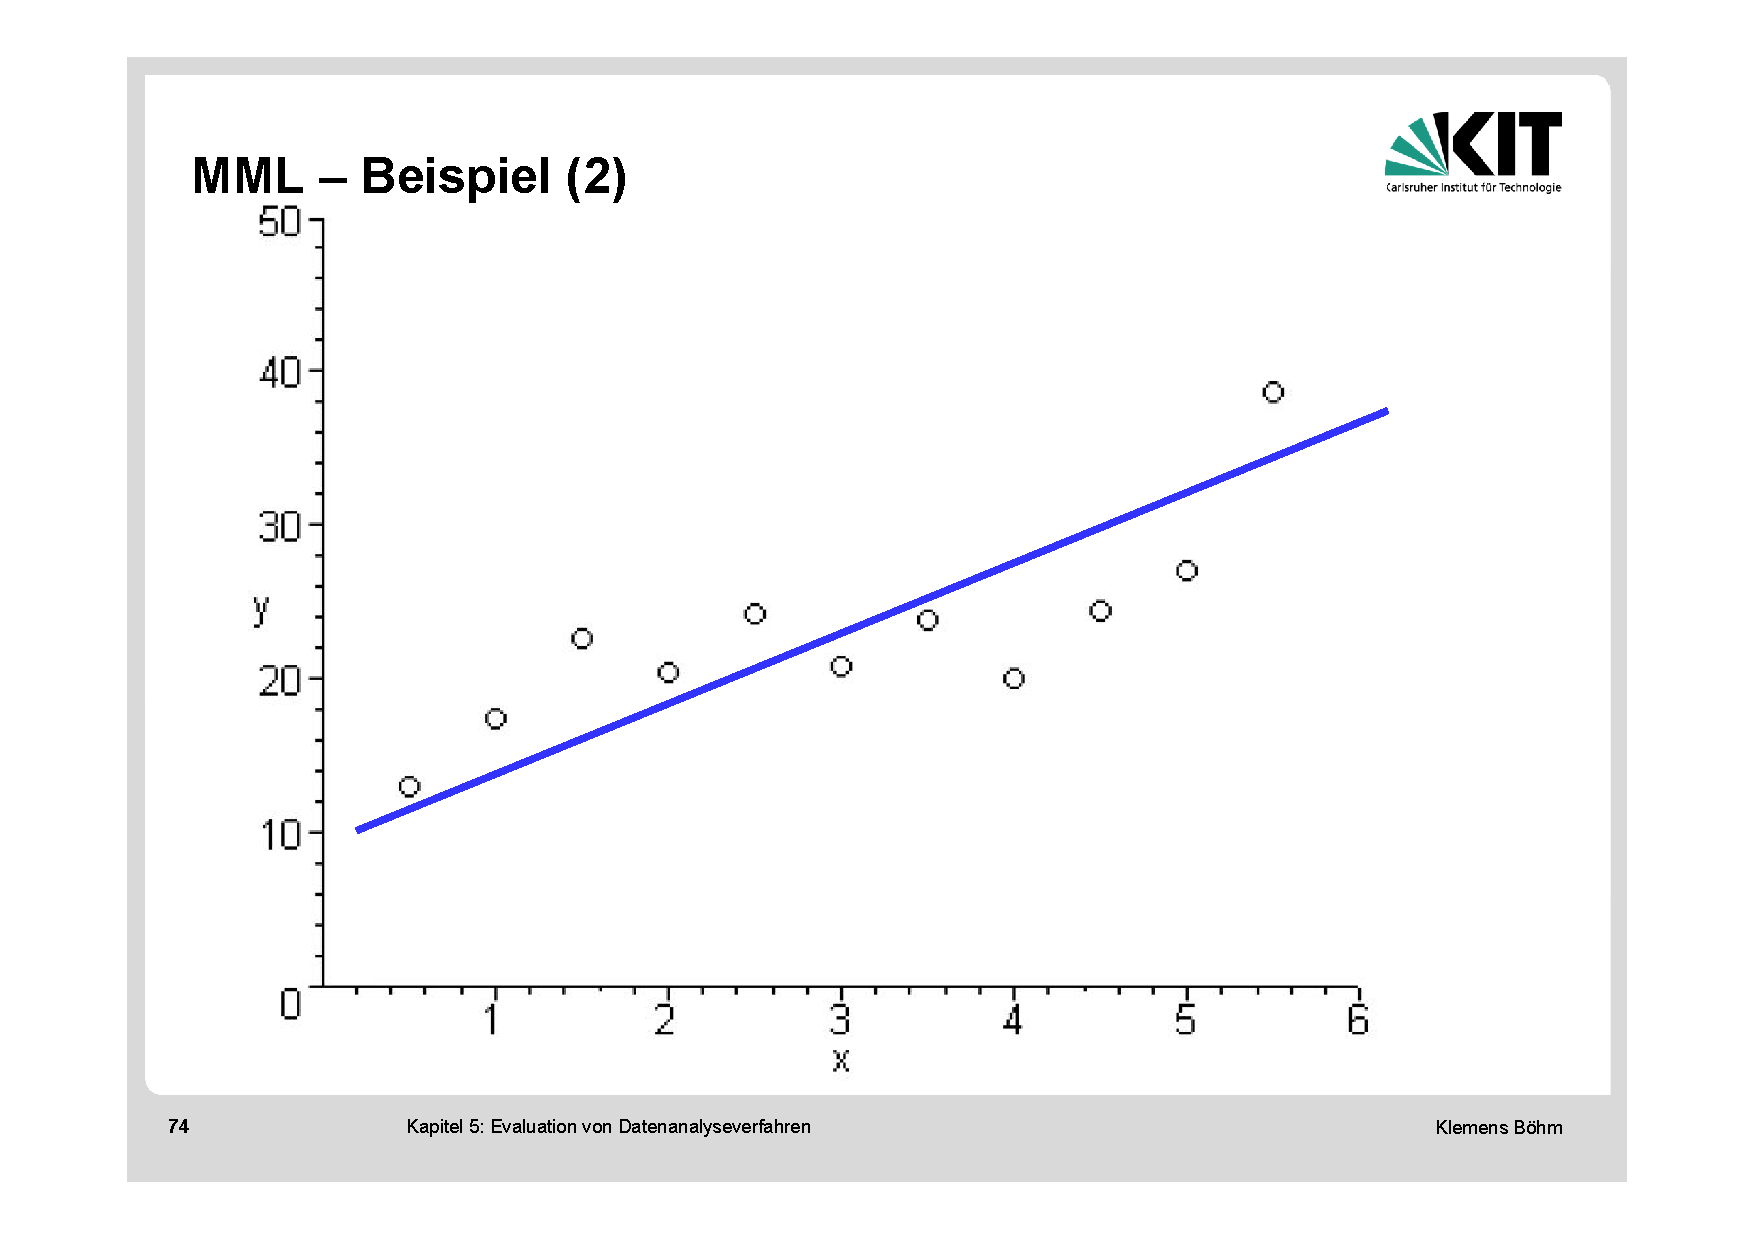
\includegraphics[width=0.49\textwidth]{Figures/mml1}}
	\subfigure[Polynomielles Modell]{
		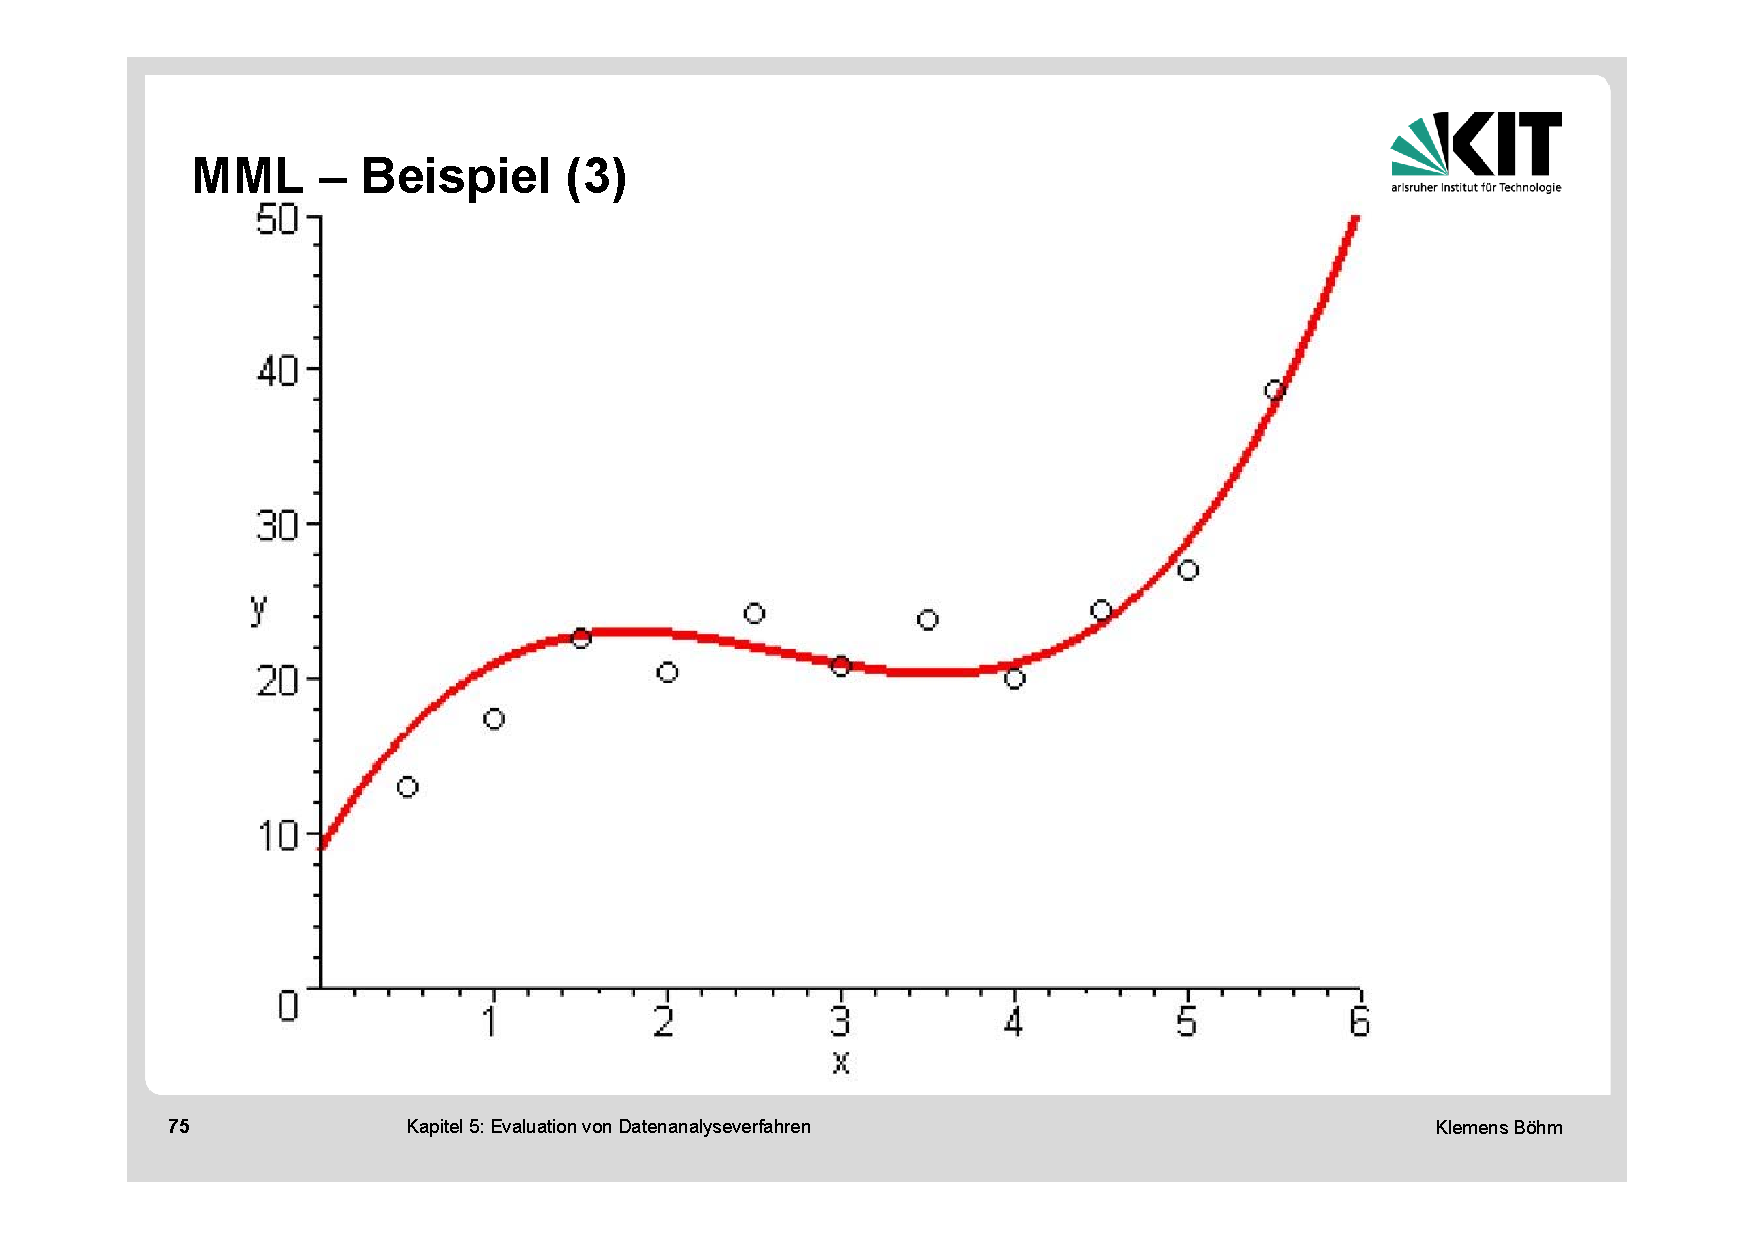
\includegraphics[width=0.49\textwidth]{Figures/mml2}}
	\caption[MML]{Beispiele von Beschreibungsmodellen für einen Datenbestand.\footnotemark}
	\label{fig:mml}
\end{figure}
\footnotetext{Foliensatz 5, S. 74,75}

Das \textbf{MDL}-Principle\footnote{In der Vorlesung auch MML-Principle.}
besagt, dass das Modell, welches die Größe des Modells zusammen mit den
zusätzlichen Informationen, die nötig sind, um die Ausnahmen vom Modell
zu beschreiben, minimiert, das geeignetste ist.
Das MDL-Principle ist eine 
Umformulierung von \textit{Ockhams Rasiermesser}\footnote{Es "'rasiert"'
unnötige Teile weg. Das ganze ist mehr eine Leitlinie mit philosophischem
Charakter, als eine echtes Theorem.}
unter Anwendung von \textit{Shannons Theorem}
\[
	length(E) = -\log_2 P(E),
\]
wobei E ein Event ist, und dem \textit{Theorem von Bayes} 
\[
	P(T\wedge E) = \frac{P(E \mid T)P(T)}{P(E)},
\]
wobei E eine feste Evidence\footnote{In der Vorlesung Examples genannt,
da man sich auf einen vorliegenden Datenbestand bezieht.}
ist und T eine Theorie beschreibt.
Wir können unser Modell und den realen Datenbestand in einer gemeinsamen
Message codieren, womit sich die Länge zu
\[
	length(T\wedge E) = -\log_2 P(T\wedge E) = -\log_2P(T) -\log_2 P(E \mid T) + \log_2P(E)
\]
ergibt. Der erste Teil steht für unser Modell, der zweite Teil codiert die 
zusätzlichen Informationen (Fehler bzw. Abweichungen),
die, wenn in das Modell eingespeist, es dem Modell
erlauben, den Datenbestand wiederherzustellen. Der letzte Teil beschreibt 
nur den Datenbestand, ist also nicht variabel und kann beim Vergleich unterschiedlicher
Theorien vernachlässigt werden. Wenn wir nun die Länge unseres Gesamtmodells (also
inkl. der Fehler) minimieren wollen, muss zum einen das Modell möglichst einfach
gehalten werden (minimiert den ersten Teil), und zum anderen jedoch den Datenbestand 
möglichst gut beschreiben können, also wenig Fehler machen (minimiert den zweiten Teil).

Sind durch \(P(T\wedge E)\) die absoluten Abweichungen kodiert, so kann dies schnell,
unhandlich werden. Deswegen kann es Sinn machen, auch die Fehler zu kodieren.
Man könnte sich eine etwaige Verteilung der Fehlerwerte zu Nutze machen, um so
die Fehler kompakt zu codieren. Somit lässt sich dann auch die Länge des Gesamtmodells
berechnen.

Die beiden Extreme an Modellen sind jene, die maximal simpel sind, dafür aber viele
Fehler machen, und solche, die perfekt an den Trainingsdatenbestand angepasst sind
(\textit{overfitting}), also keine Fehler machen, dafür aber um einiges komplexer sind.
Das MDL-Principle bestraft nun erstere Modelle dadurch, dass der zweite Teil, also
die Fehler, einen höheren Codierungsaufwand benötigt, der die Kürze des Codes im
ersten Teil zunichtemacht. Im zweiten Fall wird die Komplexität der Modelle dafür
sorgen, dass der Code insgesamt sehr lang wird.

Die Länge des Codes hängt auch davon ab, wie viele Daten betrachtet werden, da es,
je nachdem, mehr Möglichkeiten gibt, mit der Vorhersage falsch zu liegen.
So kann es bei einem kleinen Datenbestand vorteilhaft sein, ein einfaches Modell
zu wählen, da die maximale Anzahl an möglichen Fehler sehr klein ist. Im Gegensatz
dazu ist es für einen großen Bestand wichtig, ein möglichst genaues, wenngleich komplexeres
Modell zu verwenden, um die Zahl der Fehler klein zu halten.

Das MDL-Principle ist ein hochgradig abstraktes Prinzip und sieht auf dem Papier
ziemlich einfach aus. Die praktische Umsetzung ist jedoch im Allgemeinen gelinde
gesagt sau schwer. Zum einen ist die Codierung des Modells ein echtes Problem.
In Abb.~\ref{fig:mml} werden die Daten durch ein Polynom beschrieben;
hätte man sich stattdessen eines Entscheidungsbaumes bedient, so wird die
Codierung offensichtlich um einiges schwieriger. Auch die Umwandlung der 
zusätzlichen Informationen ist nicht trivial, was sich schon daraus ergibt, dass
die Daten als Menge vorliegen, also keine Reihenfolge besitzen. 
So kann schon eine "'klügere"'
Anordnung der Datenobjekte bei der Codierung (z.B. wenn bestimmte Fehler mehrmals
auftreten) zu einer kürzeren Länge führen. 

Als Beispiel für die Anwendung des MDL-Principles sei das Clustering genannt.
Beim Vergleich von verschiedenen Clustering-Ergebnissen
gibt es zunächst kein offensichtliches objektives Bewertungskriterium.
Hier kann jedoch das MDL-Principle Abhilfe verschaffen.\footnote{Das MDL-Principle
kann auf sehr viele verschieden Situationen angewandt werden, was eine seiner 
großen Stärken ist.} Angenommen, unser Verfahren generiert aus dem Bestand E insgesamt
k Cluster. Nach MDL sollte ein gutes Clustering E kompakt darstellen können. Man
kann nun für jeden Cluster den Mittelpunkt wählen und dann für jedes Element von
E die Clusterzugehörigkeit und den Abstand zum entsprechenden Mittelpunkt codieren.
Liegt in den Daten ein natürliches Clustering vor, so wird sich das in einem 
kurzen Code widerspiegeln.

Sollten hingegen nicht numerische sonder nominale Attributwerte vorliegen, so
kann man in jeden Cluster eine Wahrscheinlichkeitsverteilung für jedes Attribut
feststellen, welche auch für jeden Cluster unterschiedlich ist. Für die Elemente aus
E gilt laut \citet{Witten11} nun:
\begin{quote}
	\glqq Attribute values are coded with respect to the relevant probability
	distribution, a standard operation in data compression.\grqq
\end{quote}